%% Copyright 2019-2024 Elsevier Ltd
%% 
%% This file is part of the 'CAS Bundle'.
%% --------------------------------------
%% 
%% It may be distributed under the conditions of the LaTeX Project Public
%% License, either version 1.3c of this license or (at your option) any
%% later version.  The latest version of this license is in
%%    http://www.latex-project.org/lppl.txt
%% and version 1.3c or later is part of all distributions of LaTeX
%% version 1999/12/01 or later.
%% 
%% The list of all files belonging to the 'CAS Bundle' is
%% given in the file `manifest.txt'.
%% 
%% Template article for cas-sc documentclass for 
%% double column output.

\documentclass[a4paper,fleqn]{cas-sc}

% If the frontmatter runs over more than one page
% use the longmktitle option.

%\documentclass[a4paper,fleqn,longmktitle]{cas-sc}

%\usepackage[numbers]{natbib}
%\usepackage[authoryear]{natbib}
\usepackage[numbers,longnamesfirst]{natbib}
\usepackage{graphicx}

%%%Author macros
\def\tsc#1{\csdef{#1}{\textsc{\lowercase{#1}}\xspace}}
\tsc{WGM}
\tsc{QE}
%%%

\begin{document}
\let\WriteBookmarks\relax
\def\floatpagepagefraction{1}
\def\textpagefraction{.001}

% Short title
\shorttitle{Fine-Grained Fake News Detection: A Graph-Transformer Hybrid Approach}    

% Short author
\shortauthors{Aaron Koshy Parayil}  

% Main title of the paper
\title [mode = title]{Fine-Grained Fake News Detection Using Machine Learning: A Graph-Transformer Hybrid Approach}  

\author[1]{Aaron Koshy Parayil}

% Corresponding author indication
\cormark[1]
\fnmark[1]
\cortext[1]{Corresponding author}

% Address/affiliation
\affiliation[1]{organization={Christ University},
            addressline={Nagasandra}, 
            city={Bengaluru},
            postcode={560073}, 
            state={Karnataka},
            country={India}}

% Here goes the abstract
\begin{abstract}
Fake news detection has mostly been treated as a simple true-or-false problem. But real political statements rarely fall into just two categories — a claim can be mostly true, half true, or misleading in a specific way, and treating everything as binary throws away that detail. This is a harder problem than it sounds, especially for short political statements, which often need outside context (who said it, when, and in what setting) to judge properly. Early machine learning models like SVMs and basic CNNs struggled here, reaching only modest accuracy because they looked at word patterns without understanding the relationships between a speaker, their history, and the claim itself. Over time, researchers tried different fixes: adding fact-checker justifications as extra training text, modeling speakers and parties as a network using graph neural networks, and more recently, fine-tuning large language models like BERT, DeBERTa, and LLaMA on this task. Each approach improved results but came with trade-offs — some needed too much computing power, others didn't generalize well across different datasets, and many still couldn't explain why they reached a particular verdict. This paper reviews that progression and works toward a combined approach that uses both graph-based context (how speakers and statements are connected) and transformer-based language understanding together, rather than relying on just one. The goal is a model that handles fine-grained truth labels more accurately while staying practical enough to train and explain in real-world settings.
\end{abstract}

% Research highlights
\begin{highlights}
\item Evaluation of fine-grained fake news detection methodologies across evolving paradigms.
\item Comparison of graph-based contextual architectures and advanced transformer models.
\item Insights into parameter-efficient fine-tuning (PEFT) and cross-domain model generalization.
\end{highlights}

% Keywords
\begin{keywords}
Fake News Detection \sep Machine Learning \sep Natural Language Processing \sep Transformers \sep Graph Neural Networks
\end{keywords}

\maketitle

% Main text
\section{Introduction}\label{sec:intro}
Misinformation spreads faster than most people can fact-check it. A single false claim, once shared widely enough, can shape public opinion long before anyone gets around to correcting it — and by then, the correction rarely reaches as many people as the original claim did. This isn't a new problem, but the scale of it has changed. Social media, political speeches, and news aggregators now produce more claims per day than any team of human fact-checkers could realistically verify. That gap between how fast misinformation spreads and how slowly it gets corrected is what has pushed researchers toward automated detection systems.

Most early work on this problem treated it as a straightforward classification task: a statement is either true or false, and the job of the model is to sort one from the other. This framing is convenient for building datasets and training models, but it doesn't match how political statements actually work. A politician might state a fact correctly but leave out context that changes its meaning. A claim might be true in one situation and misleading in another. Fact-checking organizations like PolitiFact have long recognized this, which is why they rate statements on a scale — true, mostly true, half true, mostly false, false, and "pants on fire" — rather than a simple yes or no. Any detection system that ignores this scale is solving an easier, less useful version of the real problem.

Building a model that can make these finer distinctions is harder for a few reasons. Political statements are usually short, sometimes just a sentence or two, which leaves little text for a model to work with. They also depend heavily on context that isn't in the statement itself — who said it, what political party they belong to, what they've said before, and when the statement was made. A claim from a decade ago might no longer be true today, and a claim from a known unreliable source deserves more scrutiny than the same claim from someone with a track record of accuracy. Capturing this kind of contextual, relational information is something that early models, built mainly on word patterns, were never designed to do.

This has led to a shift in how researchers approach the problem. Instead of relying only on the text of a statement, newer work has looked at modeling the relationships between speakers and their statements using graph-based methods, and separately, at using large pre-trained language models to better understand the statement's meaning. Each direction has made progress, but also come with its own limitations — some approaches need far more computing power than is practical, others don't generalize well when applied to new domains or unseen speakers, and many still function as black boxes that give a verdict without explaining how they got there.

This paper first reviews how the field has evolved across these different approaches — from early feature-based models through graph neural networks to large language models with parameter-efficient tuning — and then builds on that groundwork to propose a hybrid approach that combines graph-based speaker context with transformer-based language understanding. The aim is a model that captures fine-grained truth distinctions more accurately than prior binary approaches, while remaining practical to train and reasonably transparent in how it reaches its conclusions. The rest of this paper is organized as follows: Section 2 reviews related work across the major methodological paradigms in fake news detection; subsequent sections detail the proposed methodology, experimental setup, results, and conclusions.

\section{Literature Survey}\label{sec:lit_survey}

\subsection{Why Binary Classification Falls Short}
Most of the early work in this space treated fake news detection as a two-class problem. That framing is easy to build datasets for, but it doesn't hold up once you look at how fact-checkers actually work — a statement is rarely just "true" or "false," it's somewhere on a spectrum, and where exactly it falls often depends on things outside the sentence itself: who said it, what they meant by it, and what was left out. Getting a model to make that kind of judgment call is a different and much harder problem than binary classification, and it's the one this section is really about.

\subsection{Feature-Based Models and Their Ceiling}
The LIAR dataset was put together specifically to move the field past binary labels \citep{wang2017liar} — nearly 13,000 statements rated on a six-point truth scale, along with metadata like the speaker's party and history. Running standard models like SVMs and simple CNNs on it only got multi-class accuracy to around 27\%, which says less about those models being bad and more about the task being genuinely hard once you're not just predicting true/false. A follow-up approach tried feeding in the fact-checkers' written justifications alongside the statement itself, using a BiLSTM, and pushed accuracy up to around 36\% \citep{alhindi2018where}. That's a meaningful jump, but it depends on justification text that a real-time system wouldn't have available before making a decision — so it's more useful as a proof of concept than a deployable method. Separately, a CNN-LSTM setup applied to Hindi-language news reported very high accuracy within that one language \citep{gupta2025fake}, though it's unclear how well the same setup would carry over to other languages or domains.

\subsection{Modeling Speakers as a Network}
A statement doesn't exist in isolation — who says it and what they've said before matters. One line of work tried to capture that by building a graph out of speakers, parties, and statements and framing detection as a node classification problem, using a relational GNN \citep{kirilin2019relational}. It improved on the plain text-only baselines (around 38\% accuracy) but struggled with new speakers who weren't already part of the graph — a fairly common real-world scenario. Another approach combined a transformer with a graph convolutional network and contrastive learning, getting closer to 46\% \citep{park2024graph}, though building and maintaining that graph structure adds a lot of preprocessing overhead. A different angle used a co-attention based GNN focused on user profiles \citep{khedairia2025co}, reporting much higher numbers on GossipCop and PolitiFact — though those datasets are structured differently from LIAR, so the results aren't directly comparable, and the approach is computationally heavy.

\subsection{Transformers Enter the Picture}
Once attention-based models became standard, several groups tried applying them directly to this problem. Fine-tuning BERT on the LIAR and ISOT datasets got to around 41\% multi-class accuracy \citep{khan2020fake}, though BERT's 512-token limit isn't really a constraint for short political statements — the bigger issue was still capturing context beyond the text itself. Another approach folded in metadata directly through a dual-attention and MLP fusion setup, reaching about 43.5\% \citep{yang2022multimodal}, but the approach was fragile whenever metadata fields were missing, which happens often with real-world data.

\subsection{Large Language Models and Efficient Fine-Tuning}
As models got bigger, the challenge shifted from "can it understand the text" to "how do you fine-tune something this large without breaking it." Prompt and prefix tuning on GPT-2 avoided retraining the whole model \citep{zhou2023fine}, but results were oddly sensitive to how prompts were phrased. Using DeBERTa-v3's attention mechanism gave a solid bump (about 47\%) \citep{martinez2024deberta}, at the cost of needing much more compute. LLaMA-2 and Mistral were also tested in few-shot settings without any fine-tuning at all \citep{kumar2024combating}, and while 5-shot prompting got reasonably close (around 46\%), it came with heavy inference costs from long context windows.

The most competitive results in this space so far come from combining large pretrained models with efficient fine-tuning. Fine-tuning BERT, RoBERTa, and DeBERTa reported around 48\% multi-class accuracy and close to 90\% on the simpler binary version of the task \citep{alqadi2025transfer}. A similar boost was achieved using LoRA on Mistral-7B, without touching most of the model's parameters \citep{thompson2025parameter}. Binary accuracy above 99\% was reported using lightweight adapters on top of BERT \citep{alghamdi2025abert}, though that result is specific to the binary setup and doesn't tell us much about the harder multi-class version.

\subsection{Open Problems: Generalization, Explainability, and Robustness}
Beyond raw accuracy, a few practical issues keep showing up across this line of work. Models trained on one dataset often don't transfer well to another — this was addressed directly using domain-adversarial training, getting a cross-domain F1 of about 74\% \citep{patel2025cross}. Explainability is another gap: attribution methods layered on top of DeBERTa were used to show which parts of a statement drove the model's decision \citep{nguyen2025explaining}, which matters a lot if these systems are ever going to be trusted in practice. Robustness to deliberate manipulation is also still an open question — adversarial training tested against attacks generated by GPT-4o Mini held up reasonably well, but not perfectly \citep{almansoori2025adversarial}. On the architecture side, a mixture-of-experts setup on LLaMA-3.1 routed text and metadata differently, edging accuracy up to around 49\% \citep{garcia2026hybrid}, though it needs distributed multi-GPU infrastructure that most research teams won't have. Contrastive pretraining has also been explored as a way to reduce reliance on labeled data \citep{sun2026self}, and separately, researchers have looked at what happens to model performance as political discourse shifts over time \citep{oconnor2026temporal} — a problem that's easy to ignore in a static benchmark but very real in deployment.

Taken together, the field has moved from simple feature-based models toward increasingly sophisticated graph and transformer architectures, with each step trading off accuracy against cost, generalization, or interpretability. No single approach so far handles all three well at once, which is the gap this paper tries to address. It's also worth noting that a number of the higher accuracy figures reported above — including the binary result in \citep{alqadi2025transfer} — come from simpler binary-labeled datasets such as WELFake, which don't require the model to make the finer six-way distinctions that LIAR does. That gap in difficulty is part of why this work uses LIAR specifically: it keeps the harder, more realistic version of the problem in view rather than defaulting to the easier binary setup.

\section{Proposed Methodology}\label{sec:methodology}

\subsection{Preprocessing}\label{subsec:preprocessing}
Before any modeling can happen, the raw LIAR files need to be brought into a single, clean, consistent table. This section walks through each step of that process in the order it was applied, followed by an architecture diagram summarizing the full pipeline.

\subsubsection{Data Loading and Consolidation}
The LIAR dataset ships as three separate tab-separated files — \texttt{train.tsv}, \texttt{valid.tsv}, and \texttt{test.tsv} — none of which include a header row. Column names were assigned manually based on the dataset's documentation: a statement \texttt{id}, the six-way \texttt{label}, the \texttt{statement} text itself, its \texttt{subject}, the \texttt{speaker}, their \texttt{job\_title}, \texttt{state}, and \texttt{party}, five historical credibility counts (\texttt{barely\_true\_c}, \texttt{false\_c}, \texttt{half\_true\_c}, \texttt{mostly\_true\_c}, \texttt{pants\_fire\_c}), and the \texttt{context} in which the statement was made. Each split was tagged with its origin (train/valid/test) before being concatenated into a single working dataframe. Keeping this tag was a deliberate choice — it means the original partition can always be recovered later, so the same cleaning and feature engineering pipeline only has to be written once instead of three separate times.

\subsubsection{Structural and Type Validation}
Once loaded, the combined dataframe was checked for shape, column data types, and general structural consistency. All text-based columns were stored as strings, and the five credibility count columns as floating-point numbers. A basic text cleanup pass was also run at this stage: leading and trailing whitespace was stripped from every string column, and empty strings or literal \texttt{"nan"}/\texttt{"None"} values were normalized into proper \texttt{NaN} markers. This step matters more than it sounds — pandas does not automatically treat an empty string as missing data, so skipping this cleanup would have caused later missing-value checks to undercount how much data was actually absent.

\subsubsection{Missing Value Analysis}
With the data properly typed and cleaned, the next step was to quantify how much was missing, and where. Every column was checked for null counts and the corresponding percentage of the full dataset, which made it possible to distinguish between columns with a handful of stray missing values and columns with structurally high missingness.

\subsubsection{Duplicate Detection and Removal}
The dataset was checked for duplication at three levels: fully duplicated rows, duplicated \texttt{id} values, and duplicated statement text. Deduplication itself was performed specifically on \texttt{id}, since that is the authoritative primary key carried over from the original source files. Deduplicating on statement text was deliberately avoided, since politicians often repeat the same talking points across different appearances — those are legitimate, distinct records, not database duplicates, and removing them would have discarded real data under a false assumption.

\subsubsection{Null Handling Strategy}
Rather than applying a single blanket rule to every missing value, two different strategies were used depending on the column:
\begin{itemize}
  \item \textbf{Row removal} for rows missing a core field — \texttt{label}, \texttt{statement}, \texttt{party}, or any of the five credibility count columns. These fields are essential to every downstream step, and only a small number of rows were affected, so dropping them costs almost nothing.
  \item \textbf{Imputation} for columns with much higher missingness but lower importance — \texttt{job\_title}, \texttt{state}, \texttt{context}, \texttt{subject}, and \texttt{speaker} — using an explicit \texttt{"Unknown"} category. This preserves the row (and the usable statement text and label it contains) rather than discarding a large fraction of the dataset just because one metadata field is absent.
\end{itemize}
This mixed strategy reflects a simple principle: don't throw away data you don't have to, but don't try to guess values for fields that are core to the task either.

Figure~\ref{fig:architecture} summarizes the complete pipeline described above, from the raw source files through to the final scaled, engineered dataset.

\begin{figure}[htbp]
  \centering
  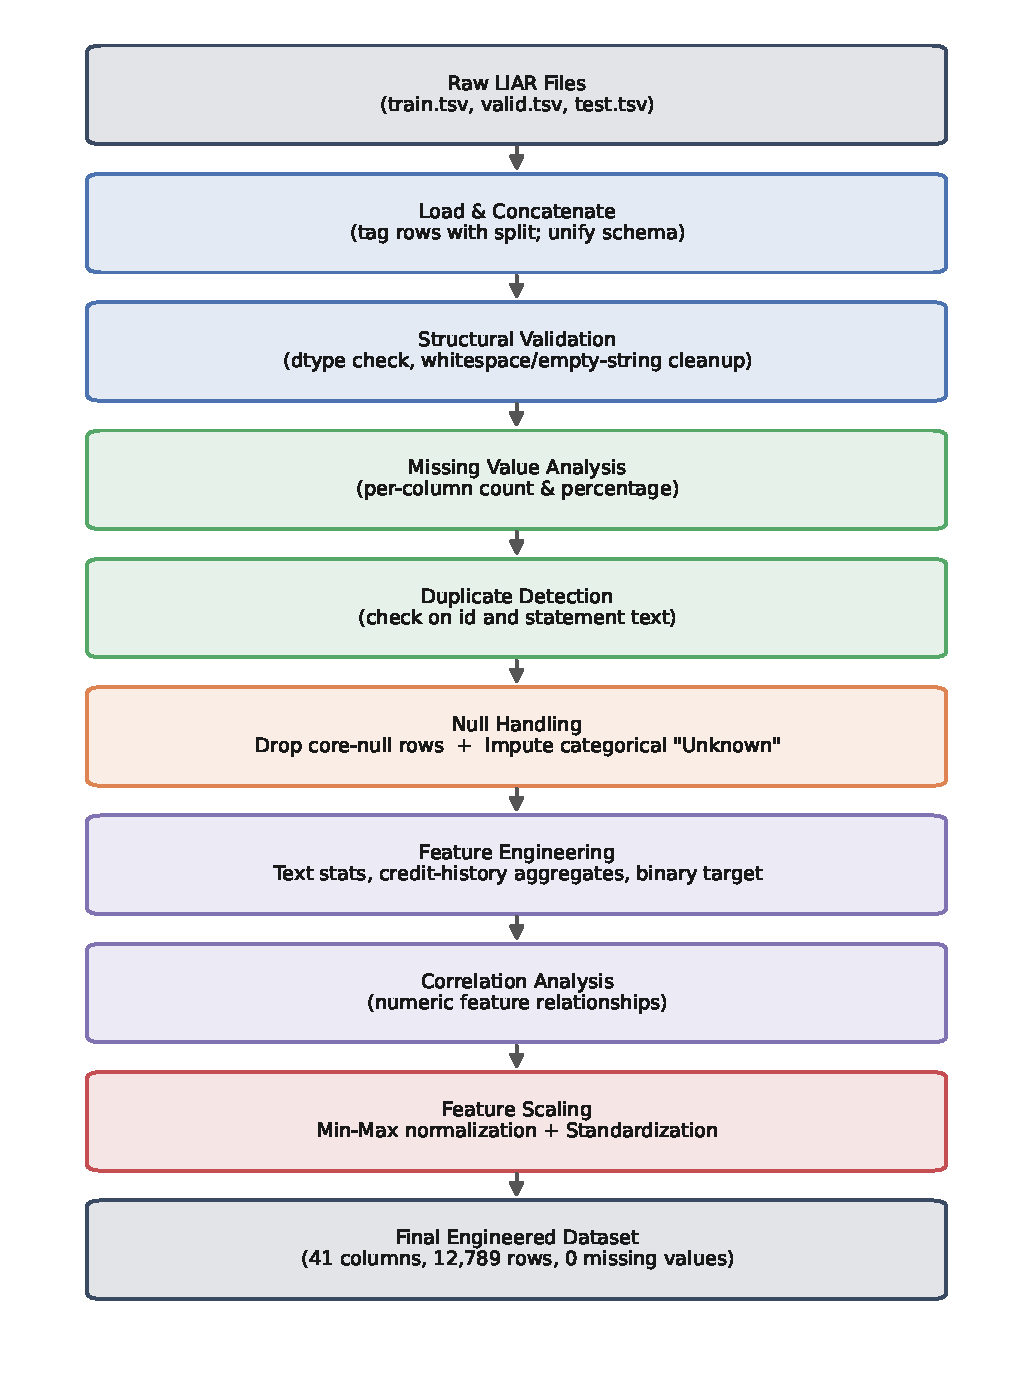
\includegraphics[width=0.75\linewidth]{figures/architecture_pipeline.pdf}
  \caption{End-to-end preprocessing and feature engineering pipeline applied to the LIAR dataset.}
  \label{fig:architecture}
\end{figure}

\subsection{Feature Engineering}\label{subsec:feature_engineering}
Once the dataset was clean and complete, a small set of derived features was constructed on top of the raw columns, split into three groups.

\textbf{Text-based features.} Three simple surface-level features were derived directly from the statement text: character length (\texttt{statement\_char\_len}), word count (\texttt{statement\_word\_count}), and average word length (\texttt{avg\_word\_length}, computed as character length divided by word count). These are cheap to compute and, as later results show, capture stylistic signal that is largely independent of the speaker's history.

\textbf{Credit-history aggregate features.} The five historical credibility counts were combined into two new features. \texttt{total\_history\_count} is simply their sum, representing how many times a speaker has been fact-checked in total, regardless of outcome. \texttt{credibility\_score} is a weighted combination of the same five counts, where truth-leaning categories are weighted positively and falsehood-leaning categories are weighted negatively — so a speaker with a long history of "mostly true" statements accumulates a higher score, while one with a long history of "false" or "pants on fire" statements accumulates a lower one. This gives a single numeric proxy for a speaker's track record, derived purely from past statements rather than the label of the current one, which keeps it safe to use as a predictive feature without leaking the target.

\textbf{Binary target.} Alongside the original six-way \texttt{label}, a simplified binary flag \texttt{is\_true} was also derived (1 for \texttt{mostly-true}/\texttt{true}, 0 otherwise). This isn't used as the primary target for this work — the whole point of using LIAR is to preserve the fine-grained distinctions — but it is retained as a secondary reference point, useful for sanity-checking models or comparing against prior binary-classification baselines.

Finally, all continuous numeric features (the five credibility counts plus the six engineered features above) were scaled two different ways: Min-Max normalization, which rescales every feature into a fixed $[0,1]$ range, and standardization (z-score scaling), which rescales each feature to zero mean and unit variance. Both scaled versions were kept as additional columns alongside the originals, so the choice of which to use can be deferred to the modeling stage — Min-Max tends to suit distance-based and neural network models, while standardization is more common for linear models.

\section{Experimental Results}\label{sec:results}

\subsection{Dataset Description}\label{subsec:dataset_description}
The LIAR dataset \citep{wang2017liar} consists of 12,791 short political statements drawn from PolitiFact, split across three files: 10,240 training statements, 1,284 validation statements, and 1,267 test statements. Each statement is labeled on a six-point truthfulness scale — \textit{pants-fire}, \textit{false}, \textit{barely-true}, \textit{half-true}, \textit{mostly-true}, and \textit{true} — and comes with speaker metadata (job title, state, party) and five historical credibility counts summarizing that speaker's prior fact-check record. After the preprocessing steps described in Section~\ref{subsec:preprocessing}, two rows with missing core fields were removed, leaving a final working dataset of 12,789 rows across 14 original columns, later expanded to 41 columns after feature engineering and scaling. No duplicate \texttt{id} values were found in the raw data, and the final dataset contains zero missing values across all columns.

\subsection{Exploratory Data Analysis (EDA)}\label{subsec:eda}

\textbf{Missing values.} Figure~\ref{fig:missing} shows the percentage of missing values per column prior to cleaning. Two columns stood out with substantial missingness: \texttt{job\_title} (27.89\% missing, 3,568 rows) and \texttt{state} (21.51\% missing, 2,751 rows). This is not surprising — not every speaker in the dataset has a formal, mapped job title or a US state on record, particularly for speakers who are organizations, media outlets, or social media posts rather than individual politicians. \texttt{context} was missing in a much smaller fraction of rows (1.02\%), while \texttt{speaker}, \texttt{subject}, \texttt{party}, and all five credibility count columns were only missing in a negligible number of rows (0.02\% each, corresponding to just 2 rows), most likely from a handful of malformed source records rather than any systematic gap.

\begin{figure}[htbp]
  \centering
  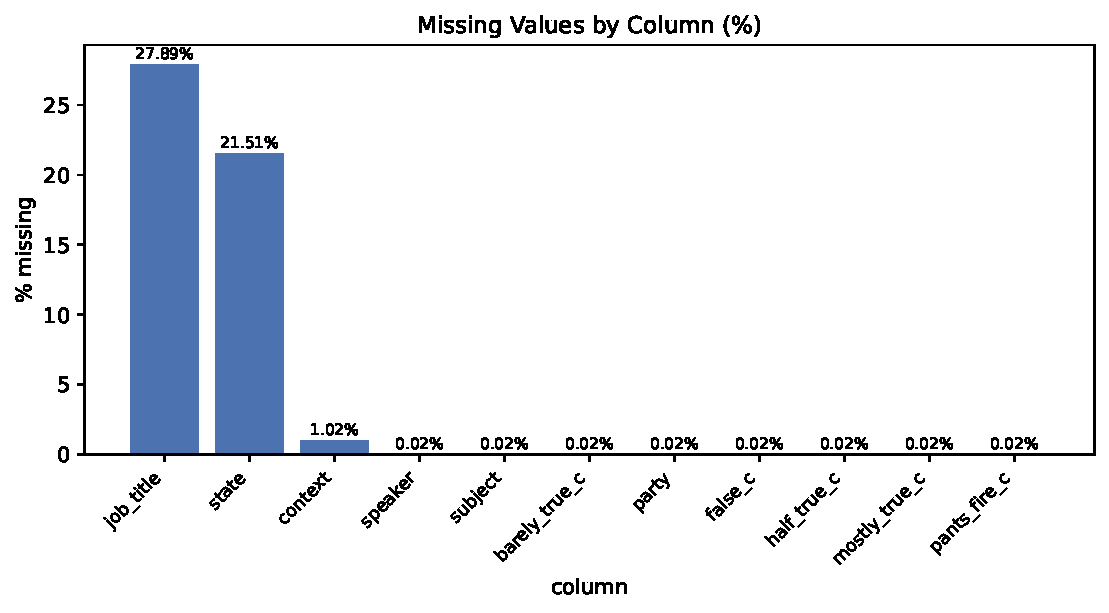
\includegraphics[width=0.95\linewidth]{figures/missing_values.pdf}
  \caption{Missing values by column, as a percentage of the full combined dataset.}
  \label{fig:missing}
\end{figure}

\textbf{Duplicates.} No fully duplicated rows and no duplicated \texttt{id} values were found. Twenty-six statements shared identical text with another row, which is expected in a dataset of political speech — the same claim or talking point is often repeated by a speaker across multiple appearances — and these were correctly retained as distinct, valid records rather than removed as duplicates.

\textbf{Null handling outcome.} After dropping the small number of rows missing core fields and imputing the high-missingness categorical columns with an explicit \texttt{"Unknown"} category, the dataset was reduced from 12,791 to 12,789 rows, with zero remaining missing values across all 15 columns. This confirms the mixed removal-and-imputation strategy achieved a fully complete table while discarding only a negligible fraction of the original data.

\textbf{Label distribution.} Figure~\ref{fig:labels} shows the distribution of the six truthfulness labels. \textit{half-true} is the most common label (2,627 statements, 20.54\%), followed closely by \textit{false} (2,505, 19.59\%) and \textit{mostly-true} (2,454, 19.19\%). \textit{barely-true} and \textit{true} sit in a similar middle range (16.44\% and 16.05\% respectively), while \textit{pants-fire} is the least common label by a clear margin (1,047 statements, 8.19\%). Overall, the distribution is close to uniform across five of the six classes, with only \textit{pants-fire} noticeably under-represented. This matters for modeling: unlike many binary fake-news datasets, which are often heavily imbalanced toward one class, LIAR's multi-class distribution does not require aggressive resampling or class-weighting to avoid a model trivially favoring the majority class — though the relative scarcity of \textit{pants-fire} statements is still worth accounting for during training.

\begin{figure}[htbp]
  \centering
  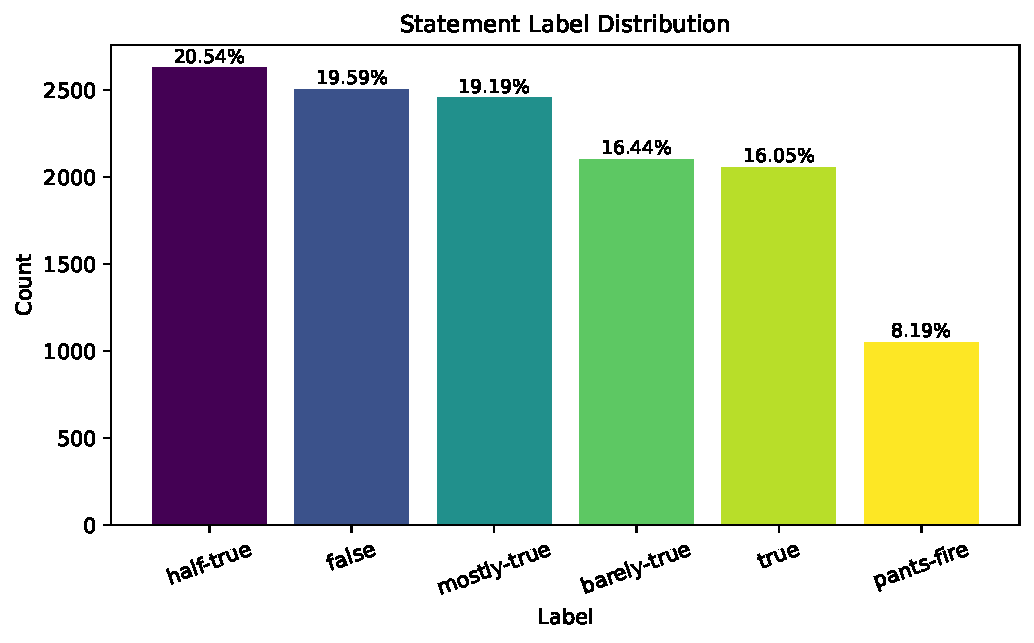
\includegraphics[width=0.95\linewidth]{figures/label_distribution.pdf}
  \caption{Distribution of the six truthfulness labels across the combined dataset.}
  \label{fig:labels}
\end{figure}

\textbf{Engineered feature statistics.} The text-based and aggregate features described in Section~\ref{subsec:feature_engineering} show a wide range of values. Statement character length averages 107.1 characters (std 63.3), ranging from as short as 11 characters to as long as 3,192. Word count follows a similar right-skewed pattern, averaging 18.0 words per statement but ranging up to 467 — the distribution is heavily concentrated at the short end, with a long tail of unusually long outlier statements. Average word length is far more tightly distributed, centered around 6.0 characters per word (std 0.69), which is expected given the relatively uniform vocabulary of political speech. \texttt{total\_history\_count} varies enormously across speakers (mean 64.9, std 115.8, up to 473), reflecting the mix of first-time speakers and heavily fact-checked repeat public figures in the dataset. \texttt{credibility\_score} averages $-32.0$ (std 83.3), consistent with the dataset's construction — since more speakers accumulate a mix of true and false statements over time than maintain a spotless record, a somewhat negative average score is expected under this weighting scheme. Finally, the binary \texttt{is\_true} flag confirms that 35.24\% of all statements fall into the \textit{mostly-true}/\textit{true} categories combined, consistent with the label distribution reported above.

A closer look at specific relationships reinforces these patterns. Credibility score, when broken out by label, rises in a clear, consistent step from \textit{pants-fire} through \textit{true} — confirming that the weighting scheme captures a real, monotonic signal about a speaker's track record rather than just noise. Party affiliation is heavily skewed toward the two major US parties, with Republican and Democrat speakers together accounting for the large majority of statements, and a smaller number attributed to independents, organizations, and other minor categories. Interestingly, average total history count does \emph{not} vary much across labels (roughly 58 to 70 statements regardless of truthfulness category) — meaning speakers with any given truthfulness profile tend to have been fact-checked a comparable number of times overall. It is specifically the \emph{composition} of that history, captured by \texttt{credibility\_score}, that differs meaningfully by label, not the raw volume of prior statements.

\textbf{Correlation analysis.} Figure~\ref{fig:corr} shows the correlation matrix across all engineered numeric features. As expected, the five raw credibility counts are all strongly correlated with one another (0.71 to 0.99), since a speaker with a long fact-checking history tends to accumulate counts across multiple categories simultaneously. \texttt{total\_history\_count} is, unsurprisingly, very strongly correlated with each of the individual counts (0.91 to 0.97), since it is their direct sum. \texttt{credibility\_score} shows a strong negative correlation with \texttt{false\_c} ($-0.70$) and an especially strong negative correlation with \texttt{pants\_fire\_c} ($-0.94$) — again expected, since these categories carry the heaviest negative weights in its construction. More interesting is what shows \emph{low} correlation: the text-based features (\texttt{statement\_char\_len}, \texttt{statement\_word\_count}, \texttt{avg\_word\_length}) are all close to uncorrelated with the credit-history features (correlations mostly under 0.05 in magnitude), which means they are contributing genuinely independent signal rather than duplicating information already present in the speaker's history. The binary target \texttt{is\_true} shows only a mild positive correlation with \texttt{credibility\_score} (0.14) and a mild negative correlation with \texttt{pants\_fire\_c} ($-0.12$) — present, but modest, which suggests that credibility history alone is informative but far from sufficient to predict truthfulness on its own, reinforcing the case for combining it with the statement's actual text content during modeling.

\begin{figure}[htbp]
  \centering
  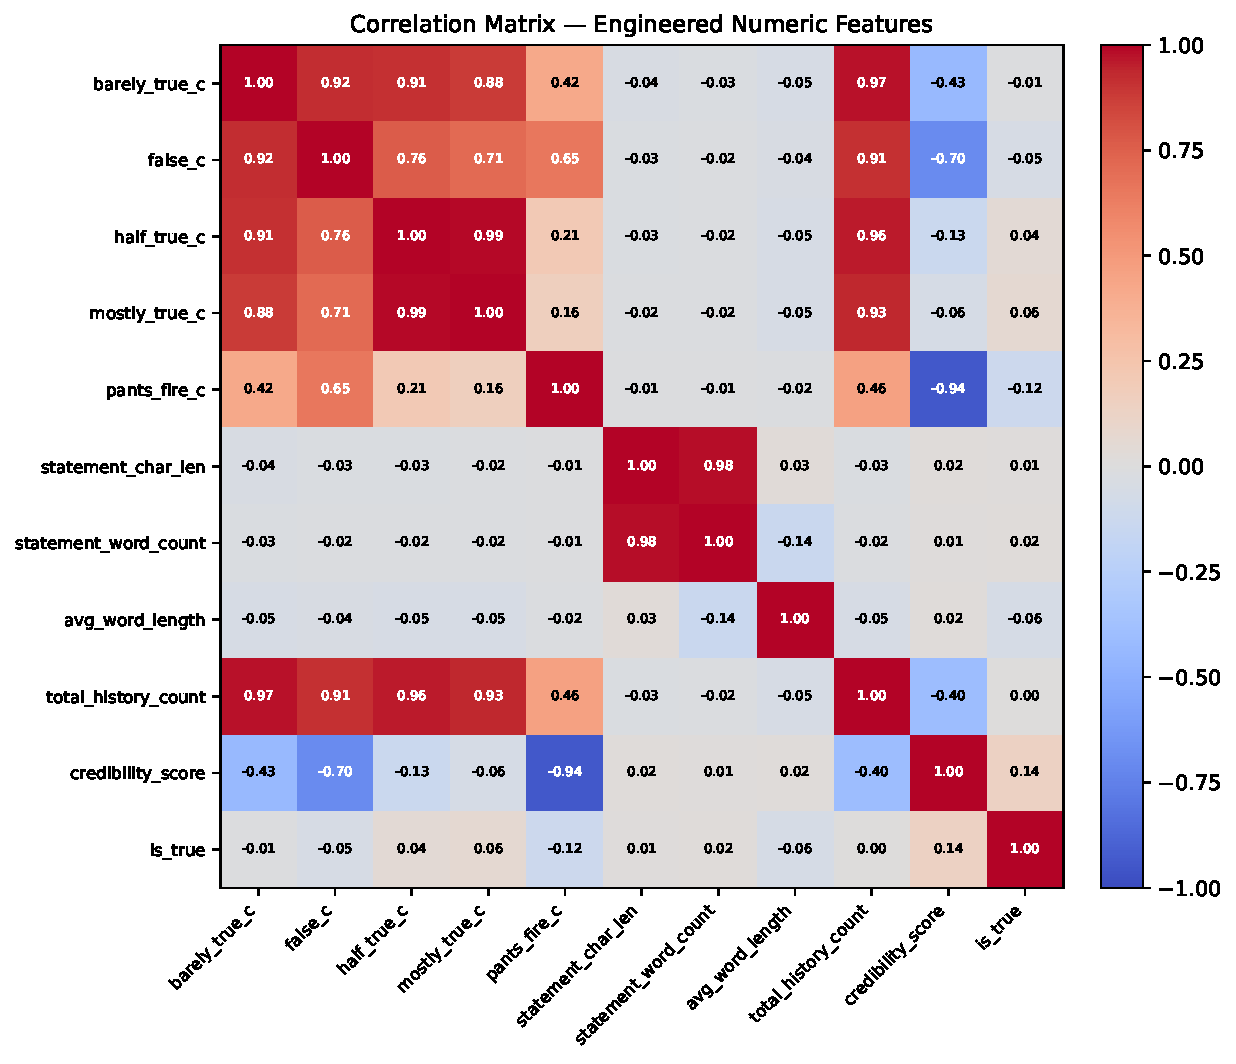
\includegraphics[width=0.98\linewidth]{figures/correlation_heatmap.pdf}
  \caption{Correlation matrix across all engineered numeric features.}
  \label{fig:corr}
\end{figure}

\textbf{Feature scaling verification.} After applying Min-Max normalization and standardization to the ten continuous numeric features, both transformations were verified directly: every Min-Max scaled column fell within the expected $[0, 1]$ range, and every standardized column had a mean of approximately 0 and a standard deviation of approximately 1. Both scaling methods preserved the underlying shape of each feature's distribution — including the right-skew visible in features like \texttt{credibility\_score} — confirming that the transformations only rescaled the axes rather than distorting the relationships within the data. This leaves both a $[0,1]$-bounded and a zero-centered version of every continuous feature available for whichever downstream model architecture is ultimately used.

\printcredits

%% Loading bibliography style file
\bibliographystyle{cas-model2-names}

% Loading bibliography database
\bibliography{cas-refs}

\end{document}